Comenzaremos considerando el problema de devolver todas las intersecciones en un conjunto de segmentos de línea horizontales y verticales. Dado que las líneas horizontales no tienen una sola coordenada X, tenemos que abandonar la idea de clasificar los objetos por X. En su lugar, tenemos la idea de un evento: una coordenada X en la que sucede algo interesante. En este caso, los tres tipos de eventos son: inicio de una línea horizontal, final de una línea horizontal y una línea vertical. A medida que se mueve la línea de barrido, mantendremos un conjunto activo de líneas horizontales cortadas por la línea de barrido, ordenadas por valor Y (las líneas rojas en la figura).

% TODO: \usepackage{graphicx} required
\begin{figure}[h!]
	\centering
	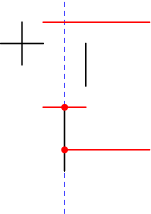
\includegraphics[width=0.2\linewidth]{img/linesvh}
	\label{fig:linesvh}
\end{figure}

Para manejar cualquiera de los eventos de línea horizontal, simplemente necesitamos agregar o eliminar un elemento del conjunto. Nuevamente, podemos usar un árbol binario balanceado para garantizar el tiempo O ($\log N$) para estas operaciones. Cuando llegamos a una línea vertical, una búsqueda de rango proporciona inmediatamente todas las líneas horizontales que corta. Si los segmentos horizontales o verticales pueden superponerse, se requiere algo de trabajo adicional, y también debemos considerar si se considera que las líneas con extremos coincidentes se cruzan, pero nada de esto afecta la complejidad computacional.

Si se requieren las intersecciones en sí, esto toma un tiempo O ($N \log N + I$) para las intersecciones $I$. Al aumentar la estructura del árbol binario (específicamente, al almacenar el tamaño de cada subárbol en la raíz de ese subárbol), es posible contar las intersecciones en tiempo O($N \log N$).

En el caso más general, las líneas no necesitan ser horizontales o verticales, por lo que las líneas en el conjunto activo pueden intercambiar lugares cuando se cruzan. En lugar de tener todos los eventos ordenados previamente, tenemos que usar una cola de prioridad y agregar y eliminar dinámicamente los eventos de intersección. En cualquier momento, la cola de prioridad contiene eventos para los puntos finales de los segmentos de línea, pero también para los puntos de intersección de los elementos adyacentes del conjunto activo (siempre que estén en el futuro). Dado que hay eventos O($N + I$) que se alcanzarán, y cada uno requiere un tiempo O($\log N$) para actualizar el conjunto activo y la cola de prioridad, este algoritmo toma un tiempo O($N \log N + I \log N$). La siguiente figura muestra los eventos futuros en la cola de prioridad (puntos azules); tenga en cuenta que no todas las intersecciones futuras están en la cola, ya sea porque una de las líneas aún no está activa o porque las dos líneas aún no son adyacentes en la lista activa.

% TODO: \usepackage{graphicx} required
\begin{figure}[h!]
	\centering
	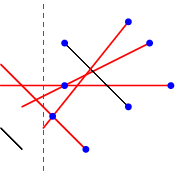
\includegraphics[width=0.2\linewidth]{img/lines}
	\label{fig:lines}
\end{figure}
